\documentclass[11pt,a4paper,final]{article}
\usepackage{stmaryrd}
\usepackage{mathbbold}
\usepackage{latexsym,bm,fancybox,enumerate}
\usepackage{geometry}
\geometry{left=2.5cm,right=2.5cm,top=2.5cm,bottom=2.5cm}
\usepackage{amsmath}
\usepackage[dvips, final]{graphicx}
\usepackage{xcolor}
\usepackage{float} % use \begin{figure}[H] to arrange the position of figure

%make the title
\newcommand{\horrule}[1]{\rule{\linewidth}{#1}} % Create horizontal rule command with 1 argument of height
\title{	
\normalfont \normalsize
\textsc{WISE, Xiamen University} \\ [25pt] % Your university, school and/or department name(s)
\horrule{0.5pt} \\[0.4cm] % Thin top horizontal rule
\huge\textbf{Statistics of Financial Markets \\
Project 4} \\ % The assignment title
\horrule{2pt} \\[0.5cm] % Thick bottom horizontal rule
}

\author{Group No. 8 \\ Group members: Li Mingyang,  Guo Junjie, Wu Heyue, Yang Buhan}

%\author{Li Mingyang \  \ 27720150150633 \\  Guo Junjie \   \ 27720150150632 \\  Wu Heyue \   \ 27720151153555  \\ Yang Buhan \  \ 15320141152125
%}

\date{\today}
\begin{document}
\maketitle
\parindent=0pt

\section{Introduction}
This is the final project of the course ''Statistics of Financial Markets''. In this project, we will apply the CIR model on term structure modeling of interest rates. The remaining parts of the project will be arranged as follows: section 2 will give a brief introduction to CIR model; section 3 shows how to apply CIR model to bond pricing; section 4 shows how to calibrate the model with actual China's spot rate data; section 5 exhibit the implied spot rate series and term structure of the model, given the estimated parameters in section 4.

\section{An Introduction to the CIR Model}
CIR model is first proposed in Cox, Ingersoll and Roll(1985). It belongs to the equilibrium spot rate model, since it is derived from a general equilibrium framework. According to the model, the motion of short-rate satisfies the following Stochastic Differential Equation (hereinafter SDE):
\begin{align}
dr(t)=a\{b-r(t)\}dt+\sigma \sqrt{r(t)}dW_t
\end{align}
where a, b, $ \sigma $ are constants and $ W_t $ is a Wiener process.

CIR model shows great merits compared to other equilibrium spot rate models: First, it incorporates mean reversion, which makes it outperform the Rendleman and Bartter��s model. Second, given $ 2ab\geq\sigma^2 $, r(t) is almost surely strictly positive, which makes it outperform the Vasicek model, where r(t) can become negative.


\section{Bond Pricing with CIR model}
Under the corresponding numeraire, the price at time t of a zero coupon bond which matures at time T can be calculated as follows:
\[
V(t,T)=E_t[exp\{-\int_{t}^{T}r(s)ds\}V(T,T)]
\]
with
\[
dr(t)=\mu_rdt+\sigma_rdW_t
\]
and $ \mu_r=\mu\{r(t),t\} $ and $ \sigma_r=\sigma\{r(t),t\} $.
By means of the terminal condition that $ V(T,T)=1 $, in combination with $ It\hat{o}'s  \,Lemma $ we get:
\[
dV(T,T)=\{\frac{\partial V(t,T)}{\partial t}+\frac{1}{2}\sigma^2\frac{\partial^2V(t,T)}{\partial r^2}+\mu_r\frac{\partial V(t,T)}{\partial r}\}dt+\sigma\frac{\partial V(t,T)}{\partial r}dW_t
\]
under the risk-neutral measure the PDE of the CIR model is:
\[
r(t)V(t,T)=\frac{\partial V(t,T)}{\partial t}+\frac{1}{2}r(t)\sigma^2\frac{\partial^2 V(t,T)}{\partial r^2}+a\{b-r(t)\}\frac{\partial V(t,T)}{\partial r}
\]
Assuming $ V(t,T)=exp\{A(t)-r(t)B(t)\} $ and a nominal value 1, we can consider:
\begin{align*}
\frac{\partial V(t,T)}{\partial t}=& \{A'(t)-r(t)B'(t)\}V(t) \\
\frac{\partial V(t,T)}{\partial r}=& -B(t)V(t) \\
\frac{\partial^2 V(t,T)}{\partial r^2}=& B^2(t)V(t)
\end{align*}
With the boundary conditions $ V(T,T)=1 $ and $ A(T,T)=B(T,T)=0 $:
\[
V(t,T)=exp\{A(t)-r(t)B(t)\}
\]
where
\begin{align*}
A(t)=& \frac{2ab}{\sigma^2}log\frac{2\psi \,exp\{(a+\psi)(T-t)/2\}}{2\psi+(a+\psi)exp\{\psi(T-t)-1\}} \\
B(t)=& \frac{2exp\{\psi(T-t)-1\}}{2\psi+(a+\psi)exp\{\psi(T-t)-1\}} \\
\psi=& \sqrt{a^2+2\sigma^2}
\end{align*}

For increasing time to maturity $ \tau $ the term structure curve $ Y_T(t) $ converges to the value:
\[
Y_{lim}=\frac{2ab}{\psi+a}
\]
and the term structure has the following properties:
\begin{itemize}
	\item $ r(t)>b $ : decreasing term structure
	\item $ r(t)<Y_{lim} $ : increasing term structure
	\item $ b>r(t)>Y_{lim} $ : term structure first rises and then falls
\end{itemize}


\section{Calibrating the CIR Model with MLE}
\subsection{Dataset}
The data we use is consist of daily observations of the annualized yield on Chinese Treasury Bond with 1 year to maturity. The time span is from 01. July 2006 to 01. July 2016. The data is downloaded from Wind Database.

\subsection{Log-likelihood function of CIR Model}
The density of $ r_{t+\Delta t} $ at time $ t+\Delta t $ is :
\[
p(r_{t+\Delta t}|r_t,\theta,\Delta t)=c\, exp(-u-v)(\frac{v}{u})^{\frac{q}{2}} \,I_q(2\sqrt{uv})
\]
where
\begin{align*}
c=& \frac{2a}{\sigma^2\{1-exp(-a\Delta t)\}} \\
u=& cr_t \,exp(-a\Delta t) \\
v=& cr_{t+\Delta t} \\
q=& 2ab/\sigma^2-1
\end{align*}
and $ I_q(2\sqrt{uv}) $ is the modified Bessel function of the first order q.

The likelihood function for interest rate time series is:
\[
L(\theta)=\prod_{t=1}^{n-1}p(r_{t+1}|r_t,\theta,\Delta t)
\]
then the log-likelihood function of the CIR process is given by:
\begin{align}
logL(\theta)=& \sum_{t=1}^{n-1}logp(r_{t+1}|r_t,\theta,\Delta t) \notag \\
=& (n-1)log\,c+\sum_{t=1}^{n-1}[-u_t-v_{t+1}+0.5q\,log\frac{v_{t+1}}{u_t}+log\{I_q(2\sqrt{u_tv_{t+1}})\}]
\end{align}
where $ u_t=cr_texp(-a\Delta t) $, and $ v_{t+1}=cr_{t+1} $.

\subsection{Initial Estimates}
Since MLE needs good starting values, we can collect the starting values for parameter by OLS.
The conditional mean function for CIR is:
\[
m(r;\theta)=E_\theta (r_t|r_{t-1}=r)=\gamma_0+\gamma_1r
\]
with
\[
\gamma_0=-b\{exp(-a\Delta t)-1\}
\]
and
\[
\gamma_1=exp(-a\Delta t)
\]

Conditional LSE for a and b are:

\begin{align*}
\hat{a}=& -\frac{1}{\Delta t}[\{n^{-1}\sum_{t=1}^{n}(r_t-\bar{r_n})(r_{t-1}-\bar{r_{n}}^{'})\}/\{n^{-1}\sum_{t=1}^{n}(r_{t-1}-\bar{r_{n}}^{'})^2\}] \\
\hat{b}=& -\frac{\bar{r_n}-exp(-a\Delta t)\bar{r_{n}}^{'}}{exp(-a\Delta t)-1}
\end{align*}
where $ \bar{r_n}=n^{-1}\sum_{t=1}^{n}r_t $ and $\bar{r_{n}}^{'}=n^{-1}\sum_{t=1}^{n}r_{t-1} $ .

Conditional second moment is:
\begin{align*}
v(r;\theta)=& E_\theta [\{r_t-E_\theta(r_t|r_{t-1}=r)\}^2|r_{t-1}=r]=\sigma^2(\eta_0+\eta_1r) \\
\eta_0=& \frac{b}{2a}\{exp(-a\Delta t)-1\}^2 \\
\eta_1=& -\frac{1}{a}exp(-a\Delta t)\{exp(-a\Delta t)-1\}
\end{align*}
Estimator for $ \sigma $:
\[
\hat{\sigma}^2=n^{-1}\sum_{t=1}^{n}\frac{\{r_t-m(r_{t-1};\hat{a},\hat{b})\}^2}{\hat{\eta_0}+\hat{\eta_1}r_{t-1}}
\]
where $ \hat{\eta_0} $ and $ \hat{\eta_1} $ are evaluated at $ (\hat{a},\hat{b}) $.

The starting values for parameter we get use the dataset are $ \hat{\theta_0}=(\hat{a_0}, \hat{b_0}, \hat{\sigma_0})=(0.3161, 0.0275, 0.0372) $.


\subsection{Estimation results}
After collecting the starting values for parameter by OLS, we maximize the log-likelihood function in equation (2) over its parameter space, then we can get
\[
\hat{\theta}=(\hat{a}, \hat{b}, \hat{\sigma})=arg\, \max \limits_\theta \,log \,L(\theta)=(0.2452, 0.0279, 0.0373)
\]


\section{Spot Rate Series and Term Structure}
Using the estimated parameters $ \hat{\theta}=(0.2452, 0.0279, 0.0373) $, we make two additional applications: first, simulate the spot series implied by our estimation; second, plot the term structure given different short-rates.

\subsection{Simulated Spot Rate}
The simulated spot rate series is shown in figure 1 as follows:

\begin{figure}[H]
	\centering
	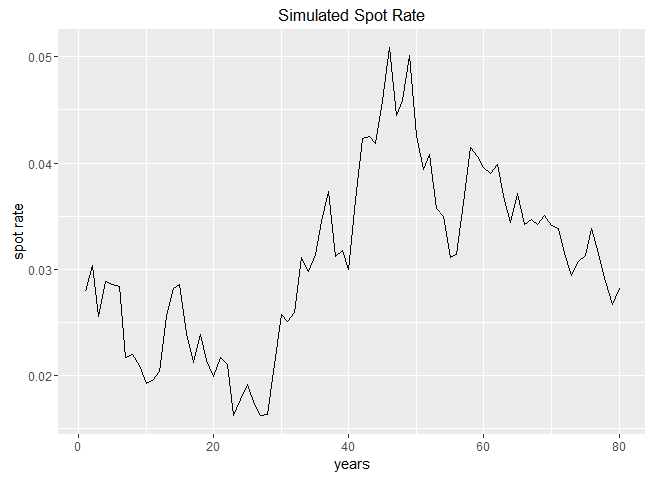
\includegraphics[height=0.4\textwidth,width=0.7\textwidth]{figure1}
	\caption{Simulated Spot Rate}
	\label{fige1}
\end{figure}

\subsection{Term Structure implied by the estimated parameters}

The properties of the term structure from section 3 states that:
\begin{itemize}
	\item $ r(t)>b $ : decreasing term structure
	\item $ r(t)<Y_{lim} $ : increasing term structure
	\item $ b>r(t)>Y_{lim} $ : term structure first rises and then falls
\end{itemize}
According to our estimation, $b=0.0279$, $Y_{lim}=\frac{2ab}{\psi+a}=0.02755$. We will check the above three properties in turn.

First, given $r(t)=0.0282 > b$, the term structure is shown in figure 2:
\begin{figure}[H]
	\centering
	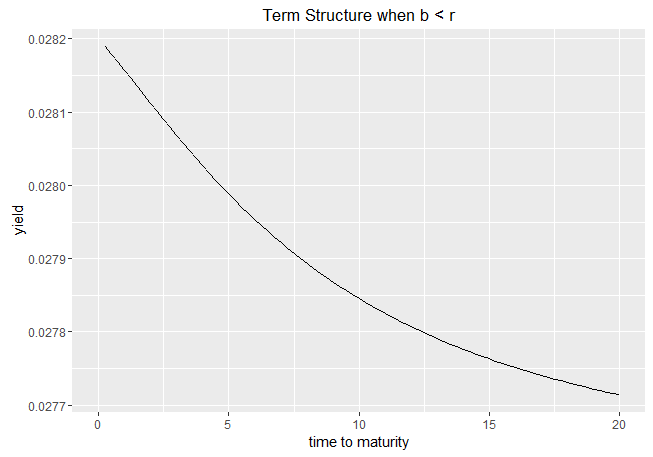
\includegraphics[height=0.4\textwidth,width=0.7\textwidth]{figure2}
	\caption{Term Structure with $ r(t)>b $}
	\label{fige2}
\end{figure}
the yield reduces as the time to maturity increases, it's consist with the statement.
\newline

Second, given $r(t)=0.0232 < Y_{lim}$, the term structure is shown in figure 3:
\begin{figure}[H]
	\centering
	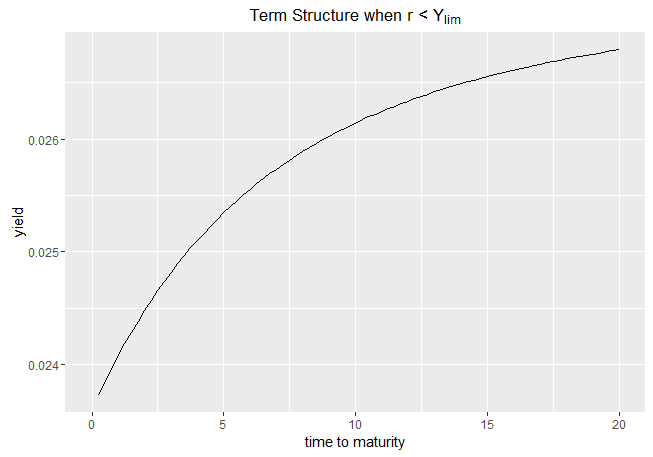
\includegraphics[height=0.4\textwidth,width=0.7\textwidth]{figure3}
	\caption{Term Structure with $ r(t)<Y_{lim} $}
	\label{fige3}
\end{figure}
Here we can see the yield rises as the time to maturity increases, it's consist with the statement too.
\newline

Third, given $ b>r(t)=0.02765>Y_{lim} $, the term structure is shown in figure 4:
\begin{figure}[H]
	\centering
	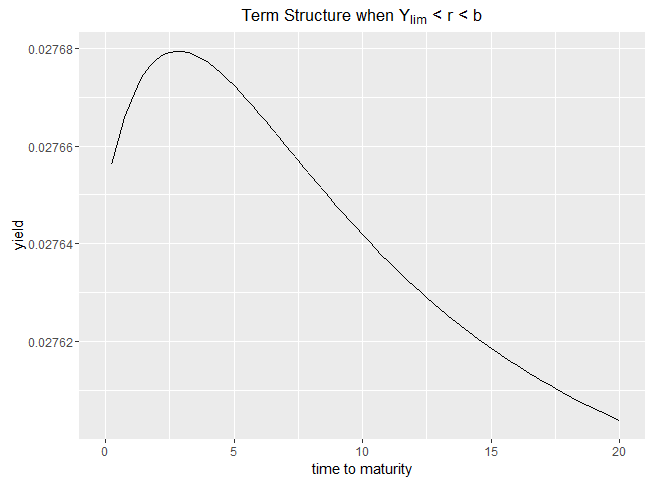
\includegraphics[height=0.4\textwidth,width=0.7\textwidth]{figure4}
	\caption{Term Structure with $ b>r(t)>Y_{lim} $}
	\label{fige4}
\end{figure}
The term structure first rises and then falls, it's consistent with the statement.


\section{References}

\begin{enumerate}
	\item Cox, J. C., Ingersoll Jr, J. E., and Ross, S. A. (1985). A theory of the term structure of interest rates. Econometrica: Journal of the Econometric Society, 385-407.
    \item Franke, J., H\"ardle, W. K., and Hafner, C. M. (2004). Statistics of financial markets (Vol. 2). Heidelberg, Germany: Springer.
    \item Hull, J. C. (2006). Options, futures, and other derivatives. Pearson Education India.
\end{enumerate}


\end{document}
